\documentclass[1p]{elsarticle_modified}
%\bibliographystyle{elsarticle-num}

%\usepackage[colorlinks]{hyperref}
%\usepackage{abbrmath_seonhwa} %\Abb, \Ascr, \Acal ,\Abf, \Afrak
\usepackage{amsfonts}
\usepackage{amssymb}
\usepackage{amsmath}
\usepackage{amsthm}
\usepackage{scalefnt}
\usepackage{amsbsy}
\usepackage{kotex}
\usepackage{caption}
\usepackage{subfig}
\usepackage{color}
\usepackage{graphicx}
\usepackage{xcolor} %% white, black, red, green, blue, cyan, magenta, yellow
\usepackage{float}
\usepackage{setspace}
\usepackage{hyperref}

\usepackage{tikz}
\usetikzlibrary{arrows}

\usepackage{multirow}
\usepackage{array} % fixed length table
\usepackage{hhline}

%%%%%%%%%%%%%%%%%%%%%
\makeatletter
\renewcommand*\env@matrix[1][\arraystretch]{%
	\edef\arraystretch{#1}%
	\hskip -\arraycolsep
	\let\@ifnextchar\new@ifnextchar
	\array{*\c@MaxMatrixCols c}}
\makeatother %https://tex.stackexchange.com/questions/14071/how-can-i-increase-the-line-spacing-in-a-matrix
%%%%%%%%%%%%%%%

\usepackage[normalem]{ulem}

\newcommand{\msout}[1]{\ifmmode\text{\sout{\ensuremath{#1}}}\else\sout{#1}\fi}
%SOURCE: \msout is \stkout macro in https://tex.stackexchange.com/questions/20609/strikeout-in-math-mode

\newcommand{\cancel}[1]{
	\ifmmode
	{\color{red}\msout{#1}}
	\else
	{\color{red}\sout{#1}}
	\fi
}

\newcommand{\add}[1]{
	{\color{blue}\uwave{#1}}
}

\newcommand{\replace}[2]{
	\ifmmode
	{\color{red}\msout{#1}}{\color{blue}\uwave{#2}}
	\else
	{\color{red}\sout{#1}}{\color{blue}\uwave{#2}}
	\fi
}

\newcommand{\Sol}{\mathcal{S}} %segment
\newcommand{\D}{D} %diagram
\newcommand{\A}{\mathcal{A}} %arc


%%%%%%%%%%%%%%%%%%%%%%%%%%%%%5 test

\def\sl{\operatorname{\textup{SL}}(2,\Cbb)}
\def\psl{\operatorname{\textup{PSL}}(2,\Cbb)}
\def\quan{\mkern 1mu \triangleright \mkern 1mu}

\theoremstyle{definition}
\newtheorem{thm}{Theorem}[section]
\newtheorem{prop}[thm]{Proposition}
\newtheorem{lem}[thm]{Lemma}
\newtheorem{ques}[thm]{Question}
\newtheorem{cor}[thm]{Corollary}
\newtheorem{defn}[thm]{Definition}
\newtheorem{exam}[thm]{Example}
\newtheorem{rmk}[thm]{Remark}
\newtheorem{alg}[thm]{Algorithm}

\newcommand{\I}{\sqrt{-1}}
\begin{document}

%\begin{frontmatter}
%
%\title{Boundary parabolic representations of knots up to 8 crossings}
%
%%% Group authors per affiliation:
%\author{Yunhi Cho} 
%\address{Department of Mathematics, University of Seoul, Seoul, Korea}
%\ead{yhcho@uos.ac.kr}
%
%
%\author{Seonhwa Kim} %\fnref{s_kim}}
%\address{Center for Geometry and Physics, Institute for Basic Science, Pohang, 37673, Korea}
%\ead{ryeona17@ibs.re.kr}
%
%\author{Hyuk Kim}
%\address{Department of Mathematical Sciences, Seoul National University, Seoul 08826, Korea}
%\ead{hyukkim@snu.ac.kr}
%
%\author{Seokbeom Yoon}
%\address{Department of Mathematical Sciences, Seoul National University, Seoul, 08826,  Korea}
%\ead{sbyoon15@snu.ac.kr}
%
%\begin{abstract}
%We find all boundary parabolic representation of knots up to 8 crossings.
%
%\end{abstract}
%\begin{keyword}
%    \MSC[2010] 57M25 
%\end{keyword}
%
%\end{frontmatter}

%\linenumbers
%\tableofcontents
%
\newcommand\colored[1]{\textcolor{white}{\rule[-0.35ex]{0.8em}{1.4ex}}\kern-0.8em\color{red} #1}%
%\newcommand\colored[1]{\textcolor{white}{ #1}\kern-2.17ex	\textcolor{white}{ #1}\kern-1.81ex	\textcolor{white}{ #1}\kern-2.15ex\color{red}#1	}

{\Large $\underline{11n_{141}~(K11n_{141})}$}

\setlength{\tabcolsep}{10pt}
\renewcommand{\arraystretch}{1.6}
\vspace{1cm}\begin{tabular}{m{100pt}>{\centering\arraybackslash}m{274pt}}
\multirow{5}{120pt}{
	\centering
	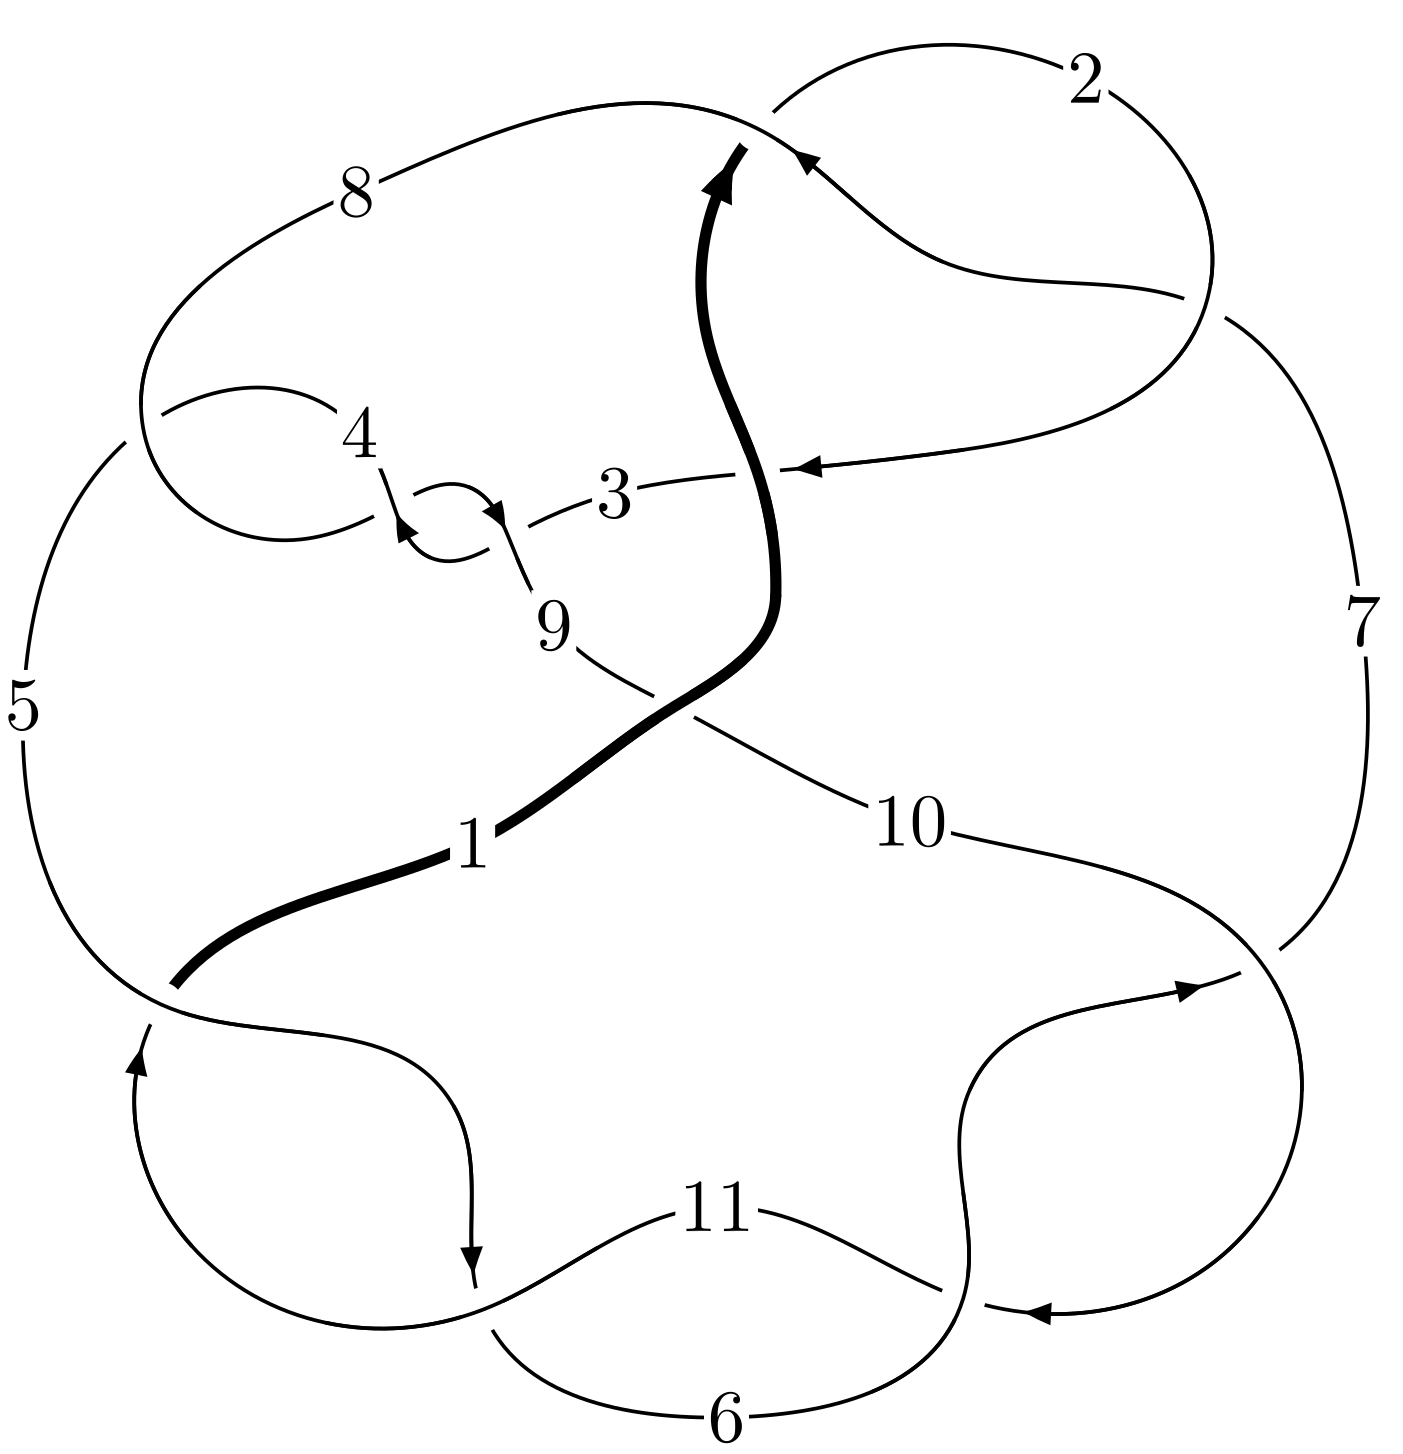
\includegraphics[width=112pt]{../../../GIT/diagram.site/Diagrams/png/757_11n_141.png}\\
\ \ \ A knot diagram\footnotemark}&
\allowdisplaybreaks
\textbf{Linearized knot diagam} \\
\cline{2-2}
 &
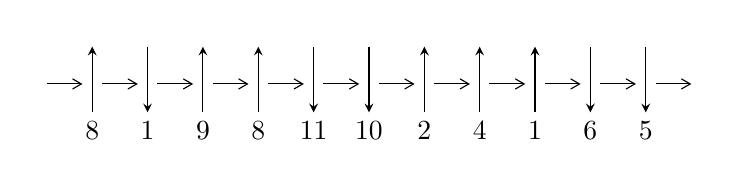
\begin{tikzpicture}[x=20pt, y=17pt]
	% nodes
	\node (C0) at (0, 0) {};
	\node (C1) at (1, 0) {};
	\node (C1U) at (1, +1) {};
	\node (C1D) at (1, -1) {8};

	\node (C2) at (2, 0) {};
	\node (C2U) at (2, +1) {};
	\node (C2D) at (2, -1) {1};

	\node (C3) at (3, 0) {};
	\node (C3U) at (3, +1) {};
	\node (C3D) at (3, -1) {9};

	\node (C4) at (4, 0) {};
	\node (C4U) at (4, +1) {};
	\node (C4D) at (4, -1) {8};

	\node (C5) at (5, 0) {};
	\node (C5U) at (5, +1) {};
	\node (C5D) at (5, -1) {11};

	\node (C6) at (6, 0) {};
	\node (C6U) at (6, +1) {};
	\node (C6D) at (6, -1) {10};

	\node (C7) at (7, 0) {};
	\node (C7U) at (7, +1) {};
	\node (C7D) at (7, -1) {2};

	\node (C8) at (8, 0) {};
	\node (C8U) at (8, +1) {};
	\node (C8D) at (8, -1) {4};

	\node (C9) at (9, 0) {};
	\node (C9U) at (9, +1) {};
	\node (C9D) at (9, -1) {1};

	\node (C10) at (10, 0) {};
	\node (C10U) at (10, +1) {};
	\node (C10D) at (10, -1) {6};

	\node (C11) at (11, 0) {};
	\node (C11U) at (11, +1) {};
	\node (C11D) at (11, -1) {5};
	\node (C12) at (12, 0) {};

	% arrows
	\draw[->,>={angle 60}]
	(C0) edge (C1) (C1) edge (C2) (C2) edge (C3) (C3) edge (C4) (C4) edge (C5) (C5) edge (C6) (C6) edge (C7) (C7) edge (C8) (C8) edge (C9) (C9) edge (C10) (C10) edge (C11) (C11) edge (C12) ;	\draw[->,>=stealth]
	(C1D) edge (C1U) (C2U) edge (C2D) (C3D) edge (C3U) (C4D) edge (C4U) (C5U) edge (C5D) (C6U) edge (C6D) (C7D) edge (C7U) (C8D) edge (C8U) (C9D) edge (C9U) (C10U) edge (C10D) (C11U) edge (C11D) ;
	\end{tikzpicture} \\
\hhline{~~} \\& 
\textbf{Solving Sequence} \\ \cline{2-2} 
 &
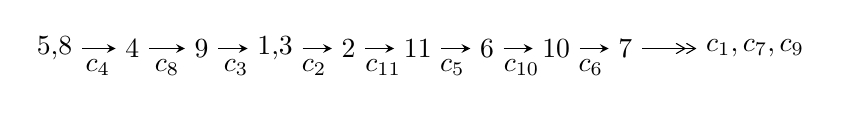
\begin{tikzpicture}[x=25pt, y=7pt]
	% node
	\node (A0) at (-1/8, 0) {5,8};
	\node (A1) at (1, 0) {4};
	\node (A2) at (2, 0) {9};
	\node (A3) at (49/16, 0) {1,3};
	\node (A4) at (33/8, 0) {2};
	\node (A5) at (41/8, 0) {11};
	\node (A6) at (49/8, 0) {6};
	\node (A7) at (57/8, 0) {10};
	\node (A8) at (65/8, 0) {7};
	\node (C1) at (1/2, -1) {$c_{4}$};
	\node (C2) at (3/2, -1) {$c_{8}$};
	\node (C3) at (5/2, -1) {$c_{3}$};
	\node (C4) at (29/8, -1) {$c_{2}$};
	\node (C5) at (37/8, -1) {$c_{11}$};
	\node (C6) at (45/8, -1) {$c_{5}$};
	\node (C7) at (53/8, -1) {$c_{10}$};
	\node (C8) at (61/8, -1) {$c_{6}$};
	\node (A9) at (10, 0) {$c_{1},c_{7},c_{9}$};

	% edge
	\draw[->,>=stealth]	
	(A0) edge (A1) (A1) edge (A2) (A2) edge (A3) (A3) edge (A4) (A4) edge (A5) (A5) edge (A6) (A6) edge (A7) (A7) edge (A8) ;
	\draw[->>,>={angle 60}]	
	(A8) edge (A9);
\end{tikzpicture} \\ 

\end{tabular} \\

\footnotetext{
The image of knot diagram is generated by the software ``\textbf{Draw programme}" developed by Andrew Bartholomew(\url{http://www.layer8.co.uk/maths/draw/index.htm\#Running-draw}), where we modified some parts for our purpose(\url{https://github.com/CATsTAILs/LinksPainter}).
}\phantom \\ \newline 
\centering \textbf{Ideals for irreducible components\footnotemark of $X_{\text{par}}$} 
 
\begin{align*}
I^u_{1}&=\langle 
- u^7- u^6-6 u^5-7 u^4-9 u^3-15 u^2+4 b-1,\;a-1,\;u^8+7 u^6+u^5+14 u^4+4 u^3+5 u^2- u+1\rangle \\
I^u_{2}&=\langle 
- u^5+2 u^4- u^3+5 u^2+5 b- u,\;u^5+2 u^3+2 u^2+5 a+u+7,\;u^6- u^5+4 u^4-4 u^3+6 u^2-4 u+5\rangle \\
I^u_{3}&=\langle 
b^2+b u+1,\;a+1,\;u^2+1\rangle \\
\\
\end{align*}
\raggedright * 3 irreducible components of $\dim_{\mathbb{C}}=0$, with total 18 representations.\\
\footnotetext{All coefficients of polynomials are rational numbers. But the coefficients are sometimes approximated in decimal forms when there is not enough margin.}
\newpage
\renewcommand{\arraystretch}{1}
\centering \section*{I. $I^u_{1}= \langle - u^7- u^6-6 u^5-7 u^4-9 u^3-15 u^2+4 b-1,\;a-1,\;u^8+7 u^6+u^5+14 u^4+4 u^3+5 u^2- u+1 \rangle$}
\flushleft \textbf{(i) Arc colorings}\\
\begin{tabular}{m{7pt} m{180pt} m{7pt} m{180pt} }
\flushright $a_{5}=$&$\begin{pmatrix}1\\0\end{pmatrix}$ \\
\flushright $a_{8}=$&$\begin{pmatrix}0\\u\end{pmatrix}$ \\
\flushright $a_{4}=$&$\begin{pmatrix}1\\u^2\end{pmatrix}$ \\
\flushright $a_{9}=$&$\begin{pmatrix}u\\u^3+u\end{pmatrix}$ \\
\flushright $a_{1}=$&$\begin{pmatrix}1\\\frac{1}{4} u^7+\frac{1}{4} u^6+\cdots+\frac{15}{4} u^2+\frac{1}{4}\end{pmatrix}$ \\
\flushright $a_{3}=$&$\begin{pmatrix}u^2+1\\u^4+2 u^2\end{pmatrix}$ \\
\flushright $a_{2}=$&$\begin{pmatrix}1\\\frac{1}{4} u^7+\frac{1}{4} u^6+\cdots+\frac{11}{4} u^2+\frac{1}{4}\end{pmatrix}$ \\
\flushright $a_{11}=$&$\begin{pmatrix}\frac{1}{4} u^7+\frac{1}{4} u^6+\cdots+\frac{15}{4} u^2+\frac{5}{4}\\\frac{1}{4} u^7+\frac{1}{4} u^6+\cdots+\frac{15}{4} u^2+\frac{1}{4}\end{pmatrix}$ \\
\flushright $a_{6}=$&$\begin{pmatrix}-\frac{1}{4} u^7+\frac{1}{4} u^6+\cdots-\frac{1}{2} u+\frac{3}{4}\\-\frac{1}{2} u^7-\frac{7}{2} u^5+\cdots-\frac{1}{2} u-\frac{1}{2}\end{pmatrix}$ \\
\flushright $a_{10}=$&$\begin{pmatrix}-\frac{1}{4} u^7+\frac{1}{4} u^6+\cdots+\frac{3}{2} u+\frac{1}{4}\\\frac{1}{2} u^5-\frac{1}{2} u^4+\cdots+2 u-\frac{1}{2}\end{pmatrix}$ \\
\flushright $a_{7}=$&$\begin{pmatrix}u\\\frac{1}{4} u^7-\frac{1}{4} u^6+\cdots-\frac{1}{2} u-\frac{1}{4}\end{pmatrix}$\\ \flushright $a_{7}=$&$\begin{pmatrix}u\\\frac{1}{4} u^7-\frac{1}{4} u^6+\cdots-\frac{1}{2} u-\frac{1}{4}\end{pmatrix}$\\&\end{tabular}
\flushleft \textbf{(ii) Obstruction class $= -1$}\\~\\
\flushleft \textbf{(iii) Cusp Shapes $= -2 u^7-2 u^6-13 u^5-15 u^4-25 u^3-30 u^2-12 u+1$}\\~\\
\newpage\renewcommand{\arraystretch}{1}
\flushleft \textbf{(iv) u-Polynomials at the component}\newline \\
\begin{tabular}{m{50pt}|m{274pt}}
Crossings & \hspace{64pt}u-Polynomials at each crossing \\
\hline $$\begin{aligned}c_{1},c_{3},c_{4}\\c_{7},c_{8}\end{aligned}$$&$\begin{aligned}
&u^8+7 u^6+u^5+14 u^4+4 u^3+5 u^2- u+1
\end{aligned}$\\
\hline $$\begin{aligned}c_{2}\end{aligned}$$&$\begin{aligned}
&u^8+14 u^7+77 u^6+205 u^5+260 u^4+140 u^3+61 u^2+9 u+1
\end{aligned}$\\
\hline $$\begin{aligned}c_{5},c_{6},c_{10}\\c_{11}\end{aligned}$$&$\begin{aligned}
&u^8+3 u^7+9 u^6+16 u^5+23 u^4+24 u^3+18 u^2+7 u+2
\end{aligned}$\\
\hline $$\begin{aligned}c_{9}\end{aligned}$$&$\begin{aligned}
&u^8+u^7+21 u^6+24 u^5+109 u^4+142 u^3-10 u^2-23 u+24
\end{aligned}$\\
\hline
\end{tabular}\\~\\
\newpage\renewcommand{\arraystretch}{1}
\flushleft \textbf{(v) Riley Polynomials at the component}\newline \\
\begin{tabular}{m{50pt}|m{274pt}}
Crossings & \hspace{64pt}Riley Polynomials at each crossing \\
\hline $$\begin{aligned}c_{1},c_{3},c_{4}\\c_{7},c_{8}\end{aligned}$$&$\begin{aligned}
&y^8+14 y^7+77 y^6+205 y^5+260 y^4+140 y^3+61 y^2+9 y+1
\end{aligned}$\\
\hline $$\begin{aligned}c_{2}\end{aligned}$$&$\begin{aligned}
&y^8-42 y^7+\cdots+41 y+1
\end{aligned}$\\
\hline $$\begin{aligned}c_{5},c_{6},c_{10}\\c_{11}\end{aligned}$$&$\begin{aligned}
&y^8+9 y^7+31 y^6+50 y^5+47 y^4+64 y^3+80 y^2+23 y+4
\end{aligned}$\\
\hline $$\begin{aligned}c_{9}\end{aligned}$$&$\begin{aligned}
&y^8+41 y^7+\cdots-1009 y+576
\end{aligned}$\\
\hline
\end{tabular}\\~\\
\newpage\flushleft \textbf{(vi) Complex Volumes and Cusp Shapes}
$$\begin{array}{c|c|c}  
\text{Solutions to }I^u_{1}& \I (\text{vol} + \sqrt{-1}CS) & \text{Cusp shape}\\
 \hline 
\begin{aligned}
u &= -0.405950 + 0.590547 I \\
a &= \phantom{-}1.00000\phantom{ +0.000000I} \\
b &= -0.00585 - 1.54991 I\end{aligned}
 & \phantom{-}6.99421 - 1.46497 I & \phantom{-}5.63406 + 4.72165 I \\ \hline\begin{aligned}
u &= -0.405950 - 0.590547 I \\
a &= \phantom{-}1.00000\phantom{ +0.000000I} \\
b &= -0.00585 + 1.54991 I\end{aligned}
 & \phantom{-}6.99421 + 1.46497 I & \phantom{-}5.63406 - 4.72165 I \\ \hline\begin{aligned}
u &= \phantom{-}0.195934 + 0.349055 I \\
a &= \phantom{-}1.00000\phantom{ +0.000000I} \\
b &= -0.218002 + 0.455338 I\end{aligned}
 & \phantom{-}0.133570 + 0.902562 I & \phantom{-}2.84755 - 7.78366 I \\ \hline\begin{aligned}
u &= \phantom{-}0.195934 - 0.349055 I \\
a &= \phantom{-}1.00000\phantom{ +0.000000I} \\
b &= -0.218002 - 0.455338 I\end{aligned}
 & \phantom{-}0.133570 - 0.902562 I & \phantom{-}2.84755 + 7.78366 I \\ \hline\begin{aligned}
u &= \phantom{-}0.33222 + 1.78481 I \\
a &= \phantom{-}1.00000\phantom{ +0.000000I} \\
b &= -0.34865 + 1.60107 I\end{aligned}
 & -9.04281 + 7.80349 I & \phantom{-}0.02756 - 3.21559 I \\ \hline\begin{aligned}
u &= \phantom{-}0.33222 - 1.78481 I \\
a &= \phantom{-}1.00000\phantom{ +0.000000I} \\
b &= -0.34865 - 1.60107 I\end{aligned}
 & -9.04281 - 7.80349 I & \phantom{-}0.02756 + 3.21559 I \\ \hline\begin{aligned}
u &= -0.12220 + 1.91634 I \\
a &= \phantom{-}1.00000\phantom{ +0.000000I} \\
b &= -0.927504 - 0.597003 I\end{aligned}
 & -16.1792 - 3.0379 I & -2.50917 + 2.22003 I \\ \hline\begin{aligned}
u &= -0.12220 - 1.91634 I \\
a &= \phantom{-}1.00000\phantom{ +0.000000I} \\
b &= -0.927504 + 0.597003 I\end{aligned}
 & -16.1792 + 3.0379 I & -2.50917 - 2.22003 I\\
 \hline 
 \end{array}$$\newpage\newpage\renewcommand{\arraystretch}{1}
\centering \section*{II. $I^u_{2}= \langle - u^5+2 u^4- u^3+5 u^2+5 b- u,\;u^5+2 u^3+2 u^2+5 a+u+7,\;u^6- u^5+4 u^4-4 u^3+6 u^2-4 u+5 \rangle$}
\flushleft \textbf{(i) Arc colorings}\\
\begin{tabular}{m{7pt} m{180pt} m{7pt} m{180pt} }
\flushright $a_{5}=$&$\begin{pmatrix}1\\0\end{pmatrix}$ \\
\flushright $a_{8}=$&$\begin{pmatrix}0\\u\end{pmatrix}$ \\
\flushright $a_{4}=$&$\begin{pmatrix}1\\u^2\end{pmatrix}$ \\
\flushright $a_{9}=$&$\begin{pmatrix}u\\u^3+u\end{pmatrix}$ \\
\flushright $a_{1}=$&$\begin{pmatrix}-\frac{1}{5} u^5-\frac{2}{5} u^3+\cdots-\frac{1}{5} u-\frac{7}{5}\\\frac{1}{5} u^5-\frac{2}{5} u^4+\frac{1}{5} u^3- u^2+\frac{1}{5} u\end{pmatrix}$ \\
\flushright $a_{3}=$&$\begin{pmatrix}u^2+1\\u^4+2 u^2\end{pmatrix}$ \\
\flushright $a_{2}=$&$\begin{pmatrix}-\frac{1}{5} u^5-\frac{2}{5} u^3+\cdots-\frac{1}{5} u-\frac{7}{5}\\-1\end{pmatrix}$ \\
\flushright $a_{11}=$&$\begin{pmatrix}-\frac{2}{5} u^4-\frac{1}{5} u^3-\frac{7}{5} u^2-\frac{7}{5}\\\frac{1}{5} u^5-\frac{2}{5} u^4+\frac{1}{5} u^3- u^2+\frac{1}{5} u\end{pmatrix}$ \\
\flushright $a_{6}=$&$\begin{pmatrix}\frac{2}{5} u^5-\frac{2}{5} u^4+\cdots+\frac{7}{5} u-\frac{8}{5}\\\frac{2}{5} u^5-\frac{4}{5} u^4+\cdots+\frac{7}{5} u-2\end{pmatrix}$ \\
\flushright $a_{10}=$&$\begin{pmatrix}\frac{1}{5} u^5-\frac{1}{5} u^4+\cdots+\frac{6}{5} u-\frac{4}{5}\\\frac{1}{5} u^5-\frac{2}{5} u^4+\cdots+\frac{6}{5} u-1\end{pmatrix}$ \\
\flushright $a_{7}=$&$\begin{pmatrix}\frac{2}{5} u^5-\frac{3}{5} u^4+\cdots+\frac{12}{5} u-\frac{9}{5}\\\frac{1}{5} u^5-\frac{2}{5} u^4+\cdots+\frac{6}{5} u-1\end{pmatrix}$\\ \flushright $a_{7}=$&$\begin{pmatrix}\frac{2}{5} u^5-\frac{3}{5} u^4+\cdots+\frac{12}{5} u-\frac{9}{5}\\\frac{1}{5} u^5-\frac{2}{5} u^4+\cdots+\frac{6}{5} u-1\end{pmatrix}$\\&\end{tabular}
\flushleft \textbf{(ii) Obstruction class $= -1$}\\~\\
\flushleft \textbf{(iii) Cusp Shapes $= -\frac{4}{5} u^5+\frac{8}{5} u^4-\frac{24}{5} u^3+4 u^2-\frac{24}{5} u+2$}\\~\\
\newpage\renewcommand{\arraystretch}{1}
\flushleft \textbf{(iv) u-Polynomials at the component}\newline \\
\begin{tabular}{m{50pt}|m{274pt}}
Crossings & \hspace{64pt}u-Polynomials at each crossing \\
\hline $$\begin{aligned}c_{1},c_{3},c_{4}\\c_{7},c_{8}\end{aligned}$$&$\begin{aligned}
&u^6- u^5+4 u^4-4 u^3+6 u^2-4 u+5
\end{aligned}$\\
\hline $$\begin{aligned}c_{2}\end{aligned}$$&$\begin{aligned}
&u^6+7 u^5+20 u^4+34 u^3+44 u^2+44 u+25
\end{aligned}$\\
\hline $$\begin{aligned}c_{5},c_{6},c_{10}\\c_{11}\end{aligned}$$&$\begin{aligned}
&(u^3- u^2+2 u-1)^2
\end{aligned}$\\
\hline $$\begin{aligned}c_{9}\end{aligned}$$&$\begin{aligned}
&(u^3- u^2+1)^2
\end{aligned}$\\
\hline
\end{tabular}\\~\\
\newpage\renewcommand{\arraystretch}{1}
\flushleft \textbf{(v) Riley Polynomials at the component}\newline \\
\begin{tabular}{m{50pt}|m{274pt}}
Crossings & \hspace{64pt}Riley Polynomials at each crossing \\
\hline $$\begin{aligned}c_{1},c_{3},c_{4}\\c_{7},c_{8}\end{aligned}$$&$\begin{aligned}
&y^6+7 y^5+20 y^4+34 y^3+44 y^2+44 y+25
\end{aligned}$\\
\hline $$\begin{aligned}c_{2}\end{aligned}$$&$\begin{aligned}
&y^6-9 y^5+12 y^4+38 y^3-56 y^2+264 y+625
\end{aligned}$\\
\hline $$\begin{aligned}c_{5},c_{6},c_{10}\\c_{11}\end{aligned}$$&$\begin{aligned}
&(y^3+3 y^2+2 y-1)^2
\end{aligned}$\\
\hline $$\begin{aligned}c_{9}\end{aligned}$$&$\begin{aligned}
&(y^3- y^2+2 y-1)^2
\end{aligned}$\\
\hline
\end{tabular}\\~\\
\newpage\flushleft \textbf{(vi) Complex Volumes and Cusp Shapes}
$$\begin{array}{c|c|c}  
\text{Solutions to }I^u_{2}& \I (\text{vol} + \sqrt{-1}CS) & \text{Cusp shape}\\
 \hline 
\begin{aligned}
u &= \phantom{-}0.862082 + 0.785389 I \\
a &= -0.873959 - 0.978854 I \\
b &= \phantom{-}0.215080 - 1.307140 I\end{aligned}
 & -0.26574 + 2.82812 I & \phantom{-}1.50976 - 2.97945 I \\ \hline\begin{aligned}
u &= \phantom{-}0.862082 - 0.785389 I \\
a &= -0.873959 + 0.978854 I \\
b &= \phantom{-}0.215080 + 1.307140 I\end{aligned}
 & -0.26574 - 2.82812 I & \phantom{-}1.50976 + 2.97945 I \\ \hline\begin{aligned}
u &= -0.377439 + 1.194730 I \\
a &= -0.818504 + 0.574501 I \\
b &= \phantom{-}0.569840\phantom{ +0.000000I}\end{aligned}
 & -4.40332\phantom{ +0.000000I} & -5.01951 + 0. I\phantom{ +0.000000I} \\ \hline\begin{aligned}
u &= -0.377439 - 1.194730 I \\
a &= -0.818504 - 0.574501 I \\
b &= \phantom{-}0.569840\phantom{ +0.000000I}\end{aligned}
 & -4.40332\phantom{ +0.000000I} & -5.01951 + 0. I\phantom{ +0.000000I} \\ \hline\begin{aligned}
u &= \phantom{-}0.01536 + 1.53025 I \\
a &= -0.507537 - 0.568454 I \\
b &= \phantom{-}0.215080 + 1.307140 I\end{aligned}
 & -0.26574 - 2.82812 I & \phantom{-}1.50976 + 2.97945 I \\ \hline\begin{aligned}
u &= \phantom{-}0.01536 - 1.53025 I \\
a &= -0.507537 + 0.568454 I \\
b &= \phantom{-}0.215080 - 1.307140 I\end{aligned}
 & -0.26574 + 2.82812 I & \phantom{-}1.50976 - 2.97945 I\\
 \hline 
 \end{array}$$\newpage\newpage\renewcommand{\arraystretch}{1}
\centering \section*{III. $I^u_{3}= \langle b^2+b u+1,\;a+1,\;u^2+1 \rangle$}
\flushleft \textbf{(i) Arc colorings}\\
\begin{tabular}{m{7pt} m{180pt} m{7pt} m{180pt} }
\flushright $a_{5}=$&$\begin{pmatrix}1\\0\end{pmatrix}$ \\
\flushright $a_{8}=$&$\begin{pmatrix}0\\u\end{pmatrix}$ \\
\flushright $a_{4}=$&$\begin{pmatrix}1\\-1\end{pmatrix}$ \\
\flushright $a_{9}=$&$\begin{pmatrix}u\\0\end{pmatrix}$ \\
\flushright $a_{1}=$&$\begin{pmatrix}-1\\b\end{pmatrix}$ \\
\flushright $a_{3}=$&$\begin{pmatrix}0\\-1\end{pmatrix}$ \\
\flushright $a_{2}=$&$\begin{pmatrix}-1\\b-1\end{pmatrix}$ \\
\flushright $a_{11}=$&$\begin{pmatrix}b-1\\b\end{pmatrix}$ \\
\flushright $a_{6}=$&$\begin{pmatrix}- b u- b\\- b u-1\end{pmatrix}$ \\
\flushright $a_{10}=$&$\begin{pmatrix}b u+u\\- b+u\end{pmatrix}$ \\
\flushright $a_{7}=$&$\begin{pmatrix}- u\\b u\end{pmatrix}$\\ \flushright $a_{7}=$&$\begin{pmatrix}- u\\b u\end{pmatrix}$\\&\end{tabular}
\flushleft \textbf{(ii) Obstruction class $= 1$}\\~\\
\flushleft \textbf{(iii) Cusp Shapes $= 0$}\\~\\
\newpage\renewcommand{\arraystretch}{1}
\flushleft \textbf{(iv) u-Polynomials at the component}\newline \\
\begin{tabular}{m{50pt}|m{274pt}}
Crossings & \hspace{64pt}u-Polynomials at each crossing \\
\hline $$\begin{aligned}c_{1},c_{3},c_{4}\\c_{7},c_{8}\end{aligned}$$&$\begin{aligned}
&(u^2+1)^2
\end{aligned}$\\
\hline $$\begin{aligned}c_{2}\end{aligned}$$&$\begin{aligned}
&(u+1)^4
\end{aligned}$\\
\hline $$\begin{aligned}c_{5},c_{6},c_{10}\\c_{11}\end{aligned}$$&$\begin{aligned}
&u^4+3 u^2+1
\end{aligned}$\\
\hline $$\begin{aligned}c_{9}\end{aligned}$$&$\begin{aligned}
&(u^2- u-1)^2
\end{aligned}$\\
\hline
\end{tabular}\\~\\
\newpage\renewcommand{\arraystretch}{1}
\flushleft \textbf{(v) Riley Polynomials at the component}\newline \\
\begin{tabular}{m{50pt}|m{274pt}}
Crossings & \hspace{64pt}Riley Polynomials at each crossing \\
\hline $$\begin{aligned}c_{1},c_{3},c_{4}\\c_{7},c_{8}\end{aligned}$$&$\begin{aligned}
&(y+1)^4
\end{aligned}$\\
\hline $$\begin{aligned}c_{2}\end{aligned}$$&$\begin{aligned}
&(y-1)^4
\end{aligned}$\\
\hline $$\begin{aligned}c_{5},c_{6},c_{10}\\c_{11}\end{aligned}$$&$\begin{aligned}
&(y^2+3 y+1)^2
\end{aligned}$\\
\hline $$\begin{aligned}c_{9}\end{aligned}$$&$\begin{aligned}
&(y^2-3 y+1)^2
\end{aligned}$\\
\hline
\end{tabular}\\~\\
\newpage\flushleft \textbf{(vi) Complex Volumes and Cusp Shapes}
$$\begin{array}{c|c|c}  
\text{Solutions to }I^u_{3}& \I (\text{vol} + \sqrt{-1}CS) & \text{Cusp shape}\\
 \hline 
\begin{aligned}
u &= \phantom{-0.000000 -}1.000000 I \\
a &= -1.00000\phantom{ +0.000000I} \\
b &= \phantom{-0.000000 -}0.618034 I\end{aligned}
 & -2.30291\phantom{ +0.000000I} & \phantom{-0.000000 } 0 \\ \hline\begin{aligned}
u &= \phantom{-0.000000 -}1.000000 I \\
a &= -1.00000\phantom{ +0.000000I} \\
b &= \phantom{-0.000000 } -1.61803 I\end{aligned}
 & \phantom{-}5.59278\phantom{ +0.000000I} & \phantom{-0.000000 } 0 \\ \hline\begin{aligned}
u &= \phantom{-0.000000 } -1.000000 I \\
a &= -1.00000\phantom{ +0.000000I} \\
b &= \phantom{-0.000000 } -0.618034 I\end{aligned}
 & -2.30291\phantom{ +0.000000I} & \phantom{-0.000000 } 0 \\ \hline\begin{aligned}
u &= \phantom{-0.000000 } -1.000000 I \\
a &= -1.00000\phantom{ +0.000000I} \\
b &= \phantom{-0.000000 -}1.61803 I\end{aligned}
 & \phantom{-}5.59278\phantom{ +0.000000I} & \phantom{-0.000000 } 0\\
 \hline 
 \end{array}$$\newpage
\newpage\renewcommand{\arraystretch}{1}
\centering \section*{ IV. u-Polynomials}
\begin{tabular}{m{50pt}|m{274pt}}
Crossings & \hspace{64pt}u-Polynomials at each crossing \\
\hline $$\begin{aligned}c_{1},c_{3},c_{4}\\c_{7},c_{8}\end{aligned}$$&$\begin{aligned}
&(u^2+1)^2(u^6- u^5+4 u^4-4 u^3+6 u^2-4 u+5)\\
&\cdot(u^8+7 u^6+u^5+14 u^4+4 u^3+5 u^2- u+1)
\end{aligned}$\\
\hline $$\begin{aligned}c_{2}\end{aligned}$$&$\begin{aligned}
&(u+1)^4(u^6+7 u^5+20 u^4+34 u^3+44 u^2+44 u+25)\\
&\cdot(u^8+14 u^7+77 u^6+205 u^5+260 u^4+140 u^3+61 u^2+9 u+1)
\end{aligned}$\\
\hline $$\begin{aligned}c_{5},c_{6},c_{10}\\c_{11}\end{aligned}$$&$\begin{aligned}
&(u^3- u^2+2 u-1)^2(u^4+3 u^2+1)\\
&\cdot(u^8+3 u^7+9 u^6+16 u^5+23 u^4+24 u^3+18 u^2+7 u+2)
\end{aligned}$\\
\hline $$\begin{aligned}c_{9}\end{aligned}$$&$\begin{aligned}
&(u^2- u-1)^2(u^3- u^2+1)^2\\
&\cdot(u^8+u^7+21 u^6+24 u^5+109 u^4+142 u^3-10 u^2-23 u+24)
\end{aligned}$\\
\hline
\end{tabular}\newpage\renewcommand{\arraystretch}{1}
\centering \section*{ V. Riley Polynomials}
\begin{tabular}{m{50pt}|m{274pt}}
Crossings & \hspace{64pt}Riley Polynomials at each crossing \\
\hline $$\begin{aligned}c_{1},c_{3},c_{4}\\c_{7},c_{8}\end{aligned}$$&$\begin{aligned}
&(y+1)^4(y^6+7 y^5+20 y^4+34 y^3+44 y^2+44 y+25)\\
&\cdot(y^8+14 y^7+77 y^6+205 y^5+260 y^4+140 y^3+61 y^2+9 y+1)
\end{aligned}$\\
\hline $$\begin{aligned}c_{2}\end{aligned}$$&$\begin{aligned}
&(y-1)^4(y^6-9 y^5+12 y^4+38 y^3-56 y^2+264 y+625)\\
&\cdot(y^8-42 y^7+\cdots+41 y+1)
\end{aligned}$\\
\hline $$\begin{aligned}c_{5},c_{6},c_{10}\\c_{11}\end{aligned}$$&$\begin{aligned}
&(y^2+3 y+1)^2(y^3+3 y^2+2 y-1)^2\\
&\cdot(y^8+9 y^7+31 y^6+50 y^5+47 y^4+64 y^3+80 y^2+23 y+4)
\end{aligned}$\\
\hline $$\begin{aligned}c_{9}\end{aligned}$$&$\begin{aligned}
&((y^2-3 y+1)^2)(y^3- y^2+2 y-1)^2(y^{8}+41 y^{7}+\cdots-1009 y+576)
\end{aligned}$\\
\hline
\end{tabular}
\vskip 2pc
\end{document}